\pdfbookmark{Общая характеристика работы}{characteristic}             % Закладка pdf
\section*{Общая характеристика работы}

\newcommand{\actuality}{\pdfbookmark[1]{Актуальность}{actuality}\underline{\textbf{\actualityTXT}}}
\newcommand{\progress}{\pdfbookmark[1]{Разработанность темы}{progress}\underline{\textbf{\progressTXT}}}
\newcommand{\aim}{\pdfbookmark[1]{Цели}{aim}\underline{{\textbf\aimTXT}}}
\newcommand{\tasks}{\pdfbookmark[1]{Задачи}{tasks}\underline{\textbf{\tasksTXT}}}
\newcommand{\aimtasks}{\pdfbookmark[1]{Цели и задачи}{aimtasks}\aimtasksTXT}
\newcommand{\novelty}{\pdfbookmark[1]{Научная новизна}{novelty}\underline{\textbf{\noveltyTXT}}}
\newcommand{\influence}{\pdfbookmark[1]{Практическая значимость}{influence}\underline{\textbf{\influenceTXT}}}
\newcommand{\methods}{\pdfbookmark[1]{Методология и методы исследования}{methods}\underline{\textbf{\methodsTXT}}}
\newcommand{\defpositions}{\pdfbookmark[1]{Положения, выносимые на защиту}{defpositions}\underline{\textbf{\defpositionsTXT}}}
\newcommand{\reliability}{\pdfbookmark[1]{Достоверность}{reliability}\underline{\textbf{\reliabilityTXT}}}
\newcommand{\probation}{\pdfbookmark[1]{Апробация}{probation}\underline{\textbf{\probationTXT}}}
\newcommand{\contribution}{\pdfbookmark[1]{Личный вклад}{contribution}\underline{\textbf{\contributionTXT}}}
\newcommand{\publications}{\pdfbookmark[1]{Публикации}{publications}\underline{\textbf{\publicationsTXT}}}


{\actuality} Тематическое моделирование --- метод анализа текстов, производящий мягкую кластеризацию как слов, так и документов. У тематического моделирования есть два важных свойства, отличающих его от других методов работы с текстами. 

Во-первых, тренировка модели происходит ``без учителя'': для того, чтобы обработать корпус текстов посредством тематического моделирования не требуется размеченных данных или предобученных моделей. Это позволяет использовать тематическое моделирование в задачах, использование в которых предобученных моделей затрудненно: для анализа узкоспецифических текстов или текстов на редких языках, для анализа тексто-подобных данных (программный код, тексты песен, банковские транзакции, географические данные, музыкальные произведения).

Во-вторых, результатом работы тематической модели являются \textit{темы}, описываемые вероятностными распределениями. Компоненты этих распределений --- вероятность слова с учётом темы и вероятность темы в документе --- прозрачны и играют понятную роль в модели. 
Зачастую эксперт может связать тему (как множество слов и множество документов) с каким-либо понятием из предметной области (т.е. проинтерпретировать её); такое осознание помогает пониманию структуры коллекции. Поэтому важное применение тематического моделирования --- помощь в понимании больших массивов неструктурированных данных.

Аддитивная Регуляризация Тематических это такой подход который даёт много гибкости.

\textbf{Степень разработанности темы исследования}. 

Подбор гиперпараметров. Доступность. Подстраховка от заблуждений.

Всё это является нерешёнными проблемами.

% {\progress}
% Этот раздел должен быть отдельным структурным элементом по
% ГОСТ, но он, как правило, включается в описание актуальности
% темы. Нужен он отдельным структурынм элемементом или нет ---
% смотрите другие диссертации вашего совета, скорее всего не нужен.

{\aim} данного диссертационного исследования является разработка методов построения интерпретируемых тематических моделей, применимых для широкого ряда задач. Проделанная работа опубликована на GitHub как открытая библиотека TopicNet.

Для~достижения поставленной цели решаются следующие {\tasks}:
\begin{enumerate}[beginpenalty=10000] % https://tex.stackexchange.com/a/476052/104425
  \item кластеризация интентов при помощи специального куба
  \item изучение принятых метрик интерпретируемости
  \item введение кастомных метрик качества
  \item введение кастомных регуляризаторов
  \item перформанс бэзлайна сравнивается с генсимом и рецептом Мурата
\end{enumerate}

{\novelty}
\begin{enumerate}[beginpenalty=10000] % https://tex.stackexchange.com/a/476052/104425
  \item Впервые \ldots
  \item Впервые \ldots
  \item Было выполнено оригинальное исследование \ldots
\end{enumerate}

{\influence} 
Абзац про нужность библиотеки ТопикНет

Абзац про пользу относительных коэффициентов

Абзац про применимость всего этого в таких-то задачах.


{\methods} В работе использованы методы теории вероятностей, оптимизации, NLP. Экспериментальное исследование проводится на языке Python; опубликованная на GitHub библиотека TopicNet, подытоживающая результаты исследования открыта для широкой публики и удовлетворяет принципам воспроизводимости результатов.

{\defpositions}
\begin{enumerate}[beginpenalty=10000] % https://tex.stackexchange.com/a/476052/104425
  \item Изучение репрезентативности имеющихся мер интерпретируемости
  \item Предложены относительные веса модальностей, и относительные коэффициенты сглаживания/разреживания. Обеспечивают переносимость тематических моделей. Отличаются от аналогов...
  \item Псевдорегуляризатор, обеспечивающий быстрое однопроходное вычисление векторизации документов. Отличается от аналогов тем, что улучшает многие меры качества.
  \item Концепция дерева эксперимента и кубов в библиотеке TopicNet
  \item Новая адаптивная стратегия регуляризации, реализованная как отдельный куб в TopicNet
\end{enumerate}


{\reliability} полученных результатов обеспечивается \ldots 

{\probation}
Основные результаты диссертации докладывались на следующих конференциях и семинарах:
\begin{itemize}
    \item Международная конференция по компьютерной лингвистике “Диалог”, Москва, 1 июня 2018.
    \item International Conference Recent Advances in Natural Language Processing (RANLP), Варна, 3 сентября 2019.
    \item Открытая лекция в рамках образовательного проекта Физтех.Рост, Долгопрудный, 18 октября 2019.
    \item Научный семинар про коэффициентов
    \item Научный семинар про ТопикНет
    \item OpenTalks.AI – ведущая независимая открытая конференция по искусственному интеллекту, Москва, 20 февраля 2020 года.
    \item International Conference on Language Resources and Evaluation (LREC), Марсель (должна была состоятся в мае 2020).
\end{itemize}

{\contribution} Автор принимал активное участие \ldots

\ifnumequal{\value{bibliosel}}{0}
{%%% Встроенная реализация с загрузкой файла через движок bibtex8. (При желании, внутри можно использовать обычные ссылки, наподобие `\cite{vakbib1,vakbib2}`).
    {\publications} Основные результаты по теме диссертации изложены
    в~XX~печатных изданиях,
    X из которых изданы в журналах, рекомендованных ВАК,
    X "--- в тезисах докладов.
}%
{%%% Реализация пакетом biblatex через движок biber
    \begin{refsection}[bl-author, bl-registered]
        % Это refsection=1.
        % Процитированные здесь работы:
        %  * подсчитываются, для автоматического составления фразы "Основные результаты ..."
        %  * попадают в авторскую библиографию, при usefootcite==0 и стиле `\insertbiblioauthor` или `\insertbiblioauthorgrouped`
        %  * нумеруются там в зависимости от порядка команд `\printbibliography` в этом разделе.
        %  * при использовании `\insertbiblioauthorgrouped`, порядок команд `\printbibliography` в нём должен быть тем же (см. biblio/biblatex.tex)
        %
        % Невидимый библиографический список для подсчёта количества публикаций:
        \ifxetexorluatex\selectlanguage{english}\fi
        \printbibliography[heading=nobibheading, section=1, env=countauthorvak,          keyword=biblioauthorvak]%
        \printbibliography[heading=nobibheading, section=1, env=countauthorwos,          keyword=biblioauthorwos]%
        \printbibliography[heading=nobibheading, section=1, env=countauthorscopus,       keyword=biblioauthorscopus]%
        \printbibliography[heading=nobibheading, section=1, env=countauthorconf,         keyword=biblioauthorconf]%
        \printbibliography[heading=nobibheading, section=1, env=countauthorother,        keyword=biblioauthorother]%
        \printbibliography[heading=nobibheading, section=1, env=countregistered,         keyword=biblioregistered]%
        \printbibliography[heading=nobibheading, section=1, env=countauthorpatent,       keyword=biblioauthorpatent]%
        \printbibliography[heading=nobibheading, section=1, env=countauthorprogram,      keyword=biblioauthorprogram]%
        \printbibliography[heading=nobibheading, section=1, env=countauthor,             keyword=biblioauthor]%
        \printbibliography[heading=nobibheading, section=1, env=countauthorvakscopuswos, filter=vakscopuswos]%
        \printbibliography[heading=nobibheading, section=1, env=countauthorscopuswos,    filter=scopuswos]%
        %
        \nocite{*}\ifxetexorluatex\selectlanguage{russian}\fi%
        %
        \nocite{intracoh, popov_hier, bulatov2020topicnet, thetaless, prog_cook, prog_view}
        
        {\publications} Основные результаты по теме диссертации изложены в~\arabic{citeauthor}~печатных изданиях,
        \arabic{citeauthorvak} из которых изданы в журналах, рекомендованных ВАК\sloppy%
        \ifnum \value{citeauthorscopuswos}>0%
            , \arabic{citeauthorscopuswos} "--- в~периодических научных журналах, индексируемых Web of~Science и Scopus\sloppy%
        \fi%
        \ifnum \value{citeauthorconf}>0%
            , \arabic{citeauthorconf} "--- в~тезисах докладов.
        \else%
            .
        \fi%
        \ifnum \value{citeregistered}=1%
            \ifnum \value{citeauthorpatent}=1%
                Зарегистрирован \arabic{citeauthorpatent} патент.
            \fi%
            \ifnum \value{citeauthorprogram}=1%
                Зарегистрирована \arabic{citeauthorprogram} программа для ЭВМ.
            \fi%
        \fi%
        \ifnum \value{citeregistered}>1%
            Зарегистрированы\ %
            \ifnum \value{citeauthorpatent}>0%
            \formbytotal{citeauthorpatent}{патент}{}{а}{}\sloppy%
            \ifnum \value{citeauthorprogram}=0 . \else \ и~\fi%
            \fi%
            \ifnum \value{citeauthorprogram}>0%
            \formbytotal{citeauthorprogram}{программ}{а}{ы}{} для ЭВМ.
            \fi%
        \fi%
        % К публикациям, в которых излагаются основные научные результаты диссертации на соискание учёной
        % степени, в рецензируемых изданиях приравниваются патенты на изобретения, патенты (свидетельства) на
        % полезную модель, патенты на промышленный образец, патенты на селекционные достижения, свидетельства
        % на программу для электронных вычислительных машин, базу данных, топологию интегральных микросхем,
        % зарегистрированные в установленном порядке.(в ред. Постановления Правительства РФ от 21.04.2016 N 335)
    \end{refsection}%
    \begin{refsection}[bl-author, bl-registered]
        % Это refsection=2.
        % Процитированные здесь работы:
        %  * попадают в авторскую библиографию, при usefootcite==0 и стиле `\insertbiblioauthorimportant`.
        %  * ни на что не влияют в противном случае
        \nocite{intracoh}
        \nocite{popov_hier}
        \nocite{bulatov2020topicnet}
        \nocite{thetaless}
        \nocite{prog_cook}
        \nocite{prog_view}
        
    \end{refsection}%
        %
        % Всё, что вне этих двух refsection, это refsection=0,
        %  * для диссертации - это нормальные ссылки, попадающие в обычную библиографию
        %  * для автореферата:
        %     * при usefootcite==0, ссылка корректно сработает только для источника из `external.bib`. Для своих работ --- напечатает "[0]" (и даже Warning не вылезет).
        %     * при usefootcite==1, ссылка сработает нормально. В авторской библиографии будут только процитированные в refsection=0 работы.
}


% Для добавления в список публикаций автора работ, которые не были процитированы в
% автореферате, требуется их~перечислить с использованием команды \verb!\nocite! в
% \verb!Synopsis/content.tex!.
 % Характеристика работы по структуре во введении и в автореферате не отличается (ГОСТ Р 7.0.11, пункты 5.3.1 и 9.2.1), потому её загружаем из одного и того же внешнего файла, предварительно задав форму выделения некоторым параметрам

%Диссертационная работа была выполнена при поддержке грантов \dots

\underline{\textbf{Объем и структура работы.}} Диссертация состоит из введения, двух обзорных глав, четырёх глав с результатами проведенного исследования, заключения и библиографии. Полный объём диссертации составляет 143 страницы, включая 17 рисунков и 12 таблиц. Список литературы содержит 154 наименования.

\pdfbookmark{Содержание работы}{description}                          % Закладка pdf
\section*{Содержание работы}
Во \underline{\textbf{введении}} отражается актуальность
исследований, проводимых в~рамках данной диссертационной работы,
приводится обзор научной литературы по~изучаемой проблеме,
формулируется цель, ставятся задачи работы, определяется научная новизна, практическая и теоретическая значимости представляемой работы. Приводится список публикаций автора по теме диссертации и формулируются положения, вносимые на защиту.

\underline{\textbf{Первая глава}} посвящена постановке задачи тематического моделирования. Рассмотрены основные подходы к тематическому моделированию и подробно описан математический аппарат подхода ARTM.

Задача тематического моделирования заключается в нахождении матриц $\Phi$ (задающей распределение <<вероятность слова в теме>>) и $\Theta$ (задающей распределение <<вероятность темы в документе>>), которые хорошо описывают заданную коллекцию документов. Подход ARTM позволяет находить $\Phi$ и $\Theta$, учитывающие какие-либо дополнительные требования помимо соответствия коллекции.

В рамках ARTM тематические модели строятся при помощи \textit{EM-алгоритма}, в котором текущие значения матриц $\Phi$ и $\Theta$ итеративно обновляются по определённым формулам. Введение каждого дополнительного регуляризатора приводит к появлению в этих формулах новых слагаемых специального вида и не требует каких-либо сложных дополнительных выкладок.

Область применения, уникальная для тематических моделей --- описание коллекции, дающее общее представление о тематической кластерной структуре больших объёмов данных. Зачастую исследователь ищет ответы на вопросы о структуре и природе коллекции, а не пытается оптимизировать заданную меру качества.

Приложения тематического моделирования в различных областях наталкиваются на проблемы плохой интерпретируемости тем, дублирующих, мусорных и вводящих в заблуждение тем, неустойчивости результатов моделирования. 

Большую часть этих проблем можно разрешить при помощи настройки гиперпараметров, но большинство прикладных работ либо не занимаются настройкой гиперпараметров, либо производят её слабо специфицированным образом.

Сложность подбора гиперпараметров у многокритериальных моделей вызывает необходимость как измерения, так и улучшения качества тематических моделей одновременно по множеству критериев.

\underline{\textbf{Во второй главе}} рассматриваются критерии качества тематических моделей, используемые в литературе. Особое внимание уделяется мерам качества, связанными с анализом верхних (наиболее частотных, вероятных, <<топовых>>, top-10) токенов тем.

\underline{\textbf{Третья глава}} посвящена анализу общих недостатков этих мер качества. Большинство используемых в литературе подходов к оценке
интерпретируемости укладываются в следующую схему:

\begin{enumerate}
    \item Для каждой темы выбирается какой-то небольшой набор характеризующих её токенов (как правило, это 10 верхних токенов).
    \item{Этот набор анализируется одним из двух способов:
    \begin{itemize}
        \item Проведя визуальный осмотр этих токенов, эксперт каким-то образом оценивает качество темы
        \item Для каждого элемента этого набора собирается ряд статистик совстречаемостей, на основе которого вычисляются какие-то численные показатели
    \end{itemize}
    }
\end{enumerate}

В пункте (1) вышеописанной схемы тема целиком огрубляется до конечного числа слов. Каким бы образом не проводился бы дальнейший анализ, обоснование качества тематической модели
при помощи короткого списка верхних токенов представляется проблематичным.

Рисунок \ref{fig:ch3_doc_compound_auto} демонстрирует то, что верхние токены покрывают исчезающе малую часть коллекции, и ситуация ещё более усложняется наличием дополнительного требования совместной встречаемости токенов в окне. Численные расчёты подтверждают, что когерентность отдельно взятой темы, в большинстве случаев, учитывает менее тысячной доли всего корпуса текста.

\begin{figure}
    %\begin{tabular}{p{7.5cm}p{3.5cm}}
        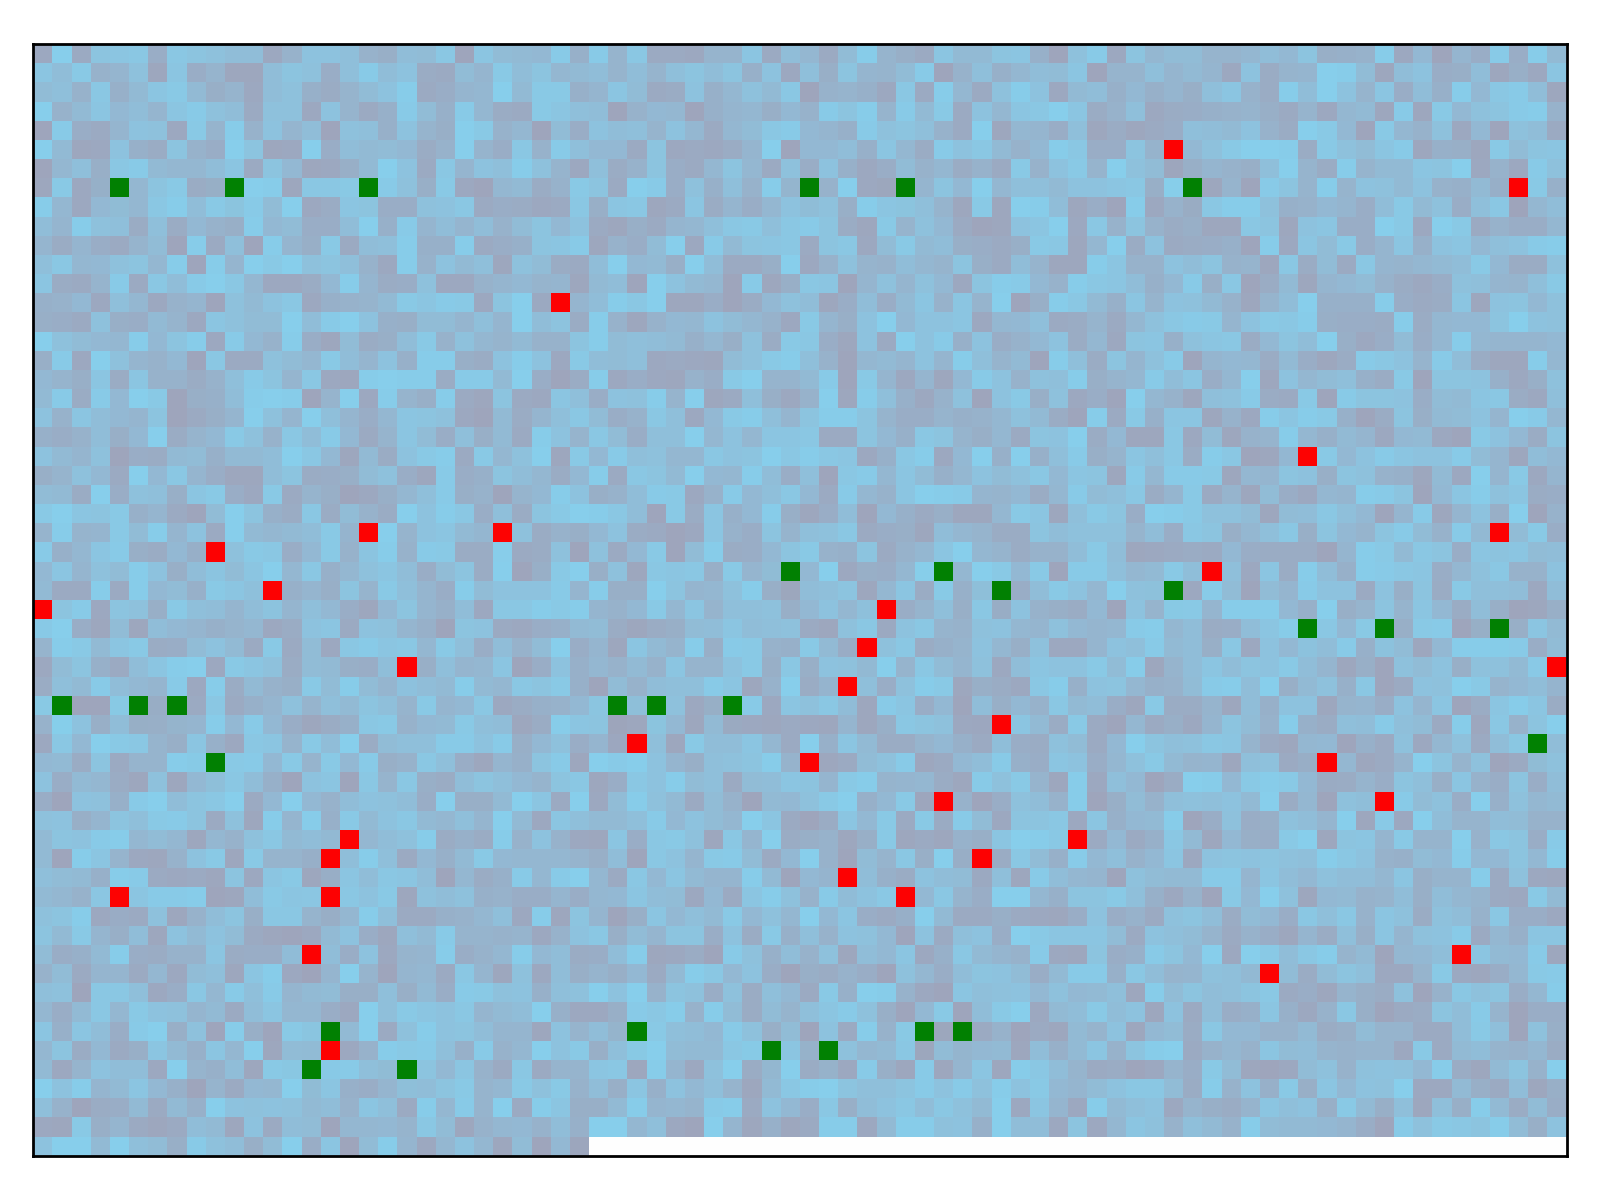
\includegraphics[width=0.75\textwidth]{doc11358_topic0.png} %&
        % 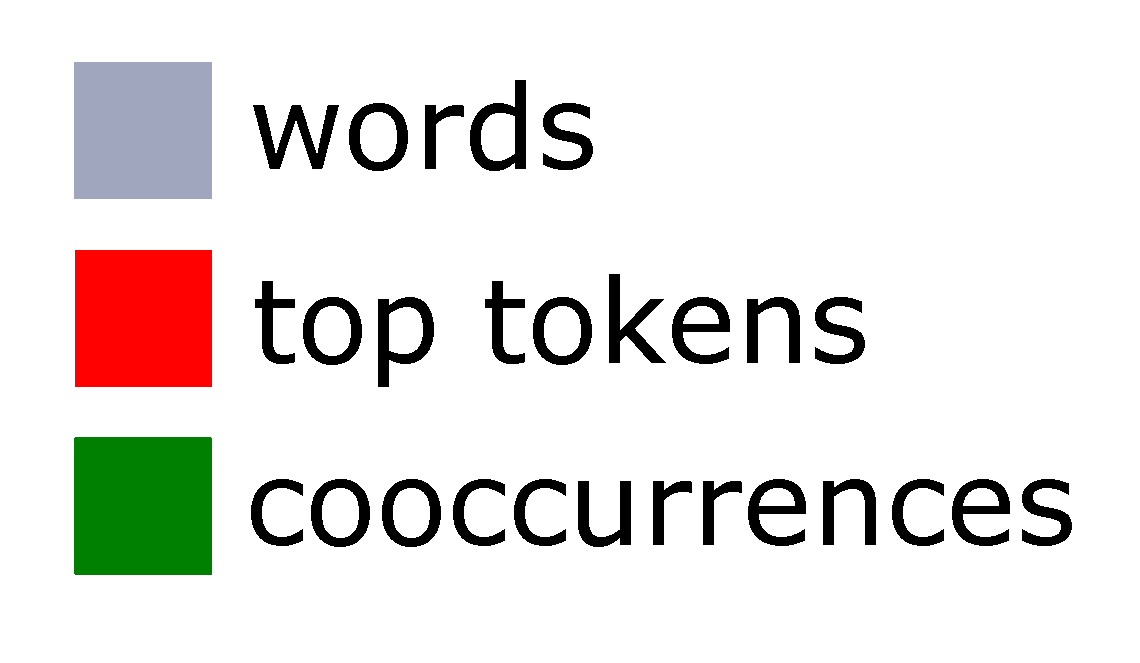
\includegraphics[width=0.25\textwidth]{legend.eps} \\
    %\end{tabular}
    \caption{Демонстрация доли текста, покрытой верхними словами, на примере одного документа. Словопозиции обозначены серо-синим цветом, словопозиции верхних слов показаны красным цветом, зелёным цветом показаны словопозиции, имеющие ненулевой вклад в расчёт когерентности (т.е. попадающие в скользящее окно вместе с другим верхним словом).}
\label{fig:ch3_doc_compound_auto}
\end{figure}

Также в этой главе предлагаются несколько мер качества, основанных на идее \textit{внутритекстовой когерентности}.
Традиционные меры когерентности сначала выделяют какое-то множество слов по их $\phi_{wt}$ и затем анализируют, каким образом эти слова встречаются в тексте (\emph{от темы к тексту}). В предлагаемом же методе сначала выделяются все соседние слова текста, распределение $\phi_{wt}$ которых затем анализируется (\emph{от текста к теме}).

Предполагается, что этот метод будет отражать коллекцию в большей степени, нежели традиционные меры когерентности. Эксперимент на полусинтетической коллекции показывает, что предлагаемый подход действительно отличается большей чувствительностью.

\underline{\textbf{В четвёртой главе}} рассматриваются способы увеличения интерпретируемости тематических моделей. Предложен метод подбора коэффициентов сглаживания, коэффициентов разреживания и весов дополнительных модальностей при помощи математического аппарата \textit{относительных коэффициентов}.

Эта техника облегчает построение тематических моделей, все темы которых различны и не <<испорчены>> большим числом неинформативных токенов (слов общей лексики). Также она позволяет перенести имеющуюсся стратегию обучения тематической модели на
другие текстовые коллекции схожей структуры.

Также в этой главе изучается псевдорегуляризатор, основанный на допущении о функциональной зависимости $\Theta = f(\Phi)$. 
Поведение предложенного алгоритма исследуется на реальных текстовых коллекциях. Результаты показывают, что этот псевдорегуляризатор повышает ряд критериев качества и успешно комбинируется с другими регуляризаторами.

\underline{\textbf{Пятая глава}} посвящена библиотеке TopicNet. TopicNet --- открытая надстройка над библиотекой BigARTM, предоставляющая более удобные
возможности для подбора гиперпараметров, для работы с пользовательскими
регуляризаторами и для визуализации тематических моделей. Описанная библиотека доступна онлайн на GitHub.

Главная мотивация TopicNet --- создать инструмент, удобный как для новичков, так и для продвинутых пользователей. Большое внимание уделяется удобству работу и наличию <<рецептов>>, показывающих хорошее качество без трудоёмкой настройки. Численный эксперимент показывает, что TopicNet с настройками <<по умолчанию>> превосходит аналогичную библиотеку GenSim с настройками <<по умолчанию>> по критериям различности, когерентности и информативности тем.

\underline{\textbf{В шестой главе}} рассматривается задача создания таксономии коллекции диалогов контактного центра без наличия разметки. Предлагается регуляризованная тематическая модель, играющая роль первого приближения к структуре коллекции.

Предлагаемая модель является двухуровневой, то есть состоит из двух <<обычных>> тематических моделей. Модель первого уровня и модель второго ориентируются на различные признаки. Это связано с тем, что первый уровень иерархии предназначен для определения предмета диалога, а цель второго уровня иерархии --- нахождение действий, которые пытается предпринять пользователь. Существительные имеют большое влияние на темы первого уровня, а для тем второго уровня более важную роль играют глаголы.

Одна и та же стратегия обучения успешно применяется к двум разным коллекциям диалогов. Первая коллекция состоит из диалогов клиентов с представителями различными государственных организаций, а вторая представляет собой логи технической поддержки провайдера. Механизм относительных коэффициентов позволил успешно перенести веса модальностей, подобранные на первой коллекции, на вторую коллекцию.


\FloatBarrier
\pdfbookmark{Заключение}{conclusion}                                  % Закладка pdf
В \underline{\textbf{заключении}} приведены основные результаты работы, которые заключаются в следующем:
%% Согласно ГОСТ Р 7.0.11-2011:
%% 5.3.3 В заключении диссертации излагают итоги выполненного исследования, рекомендации, перспективы дальнейшей разработки темы.
%% 9.2.3 В заключении автореферата диссертации излагают итоги данного исследования, рекомендации и перспективы дальнейшей разработки темы.
\begin{enumerate}[beginpenalty=10000]
\item
    Методология построения аддитивно регуляризованных тематических моделей, обеспечивающая формирование <<рецептов моделирования>> с автоматизированным подбором гиперпараметров по множеству критериев и отличающаяся использованием относительных коэффициентов регуляризации и кубов гиперпараметров.
\item
    Архитектура библиотеки TopicNet, обеспечивающая программную реализацию данной методологии и отличающаяся использованием удобного языка описания кубов гиперпараметров и возможностью создания пользовательских регуляризаторов и метрик качества на языке Python.
\item
    Универсальный рецепт моделирования, обеспечивающий многокритериальный выбор тематических моделей для широкого класса задач, отличающийся предварительной настройкой куба гиперпараметров по набору разнородных задач тематического моделирования.
\item
    Программная реализация нового критерия когерентности, обеспечивающая его эффективное вычисление и отличающаяся более полным использованием данных о сочетаемости слов внутри текстовых документов.
%\item
%    Программная реализация псевдорегуляризатора в библиотеке TopicNet, обеспечивающего быстрое однопроходное вычисление тематических векторных представлений документов и улучшение качества тематической модели по множеству критериев.
\end{enumerate}




\pdfbookmark{Литература}{bibliography}                                % Закладка pdf

% При использовании пакета \verb!biblatex! список публикаций автора по теме диссертации формируется в разделе <<\publications>>\ файла \verb!common/characteristic.tex!  при помощи команды \verb!\nocite!

\ifdefmacro{\microtypesetup}{\microtypesetup{protrusion=false}}{} % не рекомендуется применять пакет микротипографики к автоматически генерируемому списку литературы
\urlstyle{rm}                               % ссылки URL обычным шрифтом
\ifnumequal{\value{bibliosel}}{0}{% Встроенная реализация с загрузкой файла через движок bibtex8
  \renewcommand{\bibname}{\large \bibtitleauthor}
  \nocite{*}
  \insertbiblioauthor           % Подключаем Bib-базы
  %\insertbiblioexternal   % !!! bibtex не умеет работать с несколькими библиографиями !!!
}{% Реализация пакетом biblatex через движок biber
  % Цитирования.
  %  * Порядок перечисления определяет порядок в библиографии (только внутри подраздела, если `\insertbiblioauthorgrouped`).
  %  * Если не соблюдать порядок "как для \printbibliography", нумерация в `\insertbiblioauthor` будет кривой.
  %  * Если цитировать каждый источник отдельной командой --- найти некоторые ошибки будет проще.
  %
  \nocite{intracoh, popov_hier, bulatov2020topicnet, thetaless}

  %% authorprogram
  \nocite{prog_cook}%
  \nocite{prog_stkc}%
  \nocite{prog_view}%
  %

  \ifnumgreater{\value{usefootcite}}{0}{
    \begin{refcontext}[labelprefix={}]
      \ifnum \value{bibgrouped}>0
        \insertbiblioauthorgrouped    % Вывод всех работ автора, сгруппированных по источникам
      \else
        \insertbiblioauthor      % Вывод всех работ автора
      \fi
    \end{refcontext}
  }{
  \ifnum \totvalue{citeexternal}>0
    \begin{refcontext}[labelprefix=A]
      \ifnum \value{bibgrouped}>0
        \insertbiblioauthorgrouped    % Вывод всех работ автора, сгруппированных по источникам
      \else
        \insertbiblioauthor      % Вывод всех работ автора
      \fi
    \end{refcontext}
  \else
    \ifnum \value{bibgrouped}>0
      \insertbiblioauthorgrouped    % Вывод всех работ автора, сгруппированных по источникам
    \else
      \insertbiblioauthor      % Вывод всех работ автора
    \fi
  \fi
  %  \insertbiblioauthorimportant  % Вывод наиболее значимых работ автора (определяется в файле characteristic во второй section)
  \begin{refcontext}[labelprefix={}]
      \insertbiblioexternal            % Вывод списка литературы, на которую ссылались в тексте автореферата
  \end{refcontext}
  
  % Невидимый библиографический список для подсчёта количества внешних публикаций
  % Используется, чтобы убрать приставку "А" у работ автора, если в автореферате нет
  % цитирований внешних источников.
  % \printbibliography[heading=nobibheading, section=1, keyword=biblioexternal]%
  }
}
\ifdefmacro{\microtypesetup}{\microtypesetup{protrusion=true}}{}
\urlstyle{tt}                               % возвращаем установки шрифта ссылок URL
